\section{Multi-Scale Embodied Memory for VLAs}
\label{sec:method}

In this section, we describe our proposed system for equipping VLAs with memory on multiple time scales.
For robot policies deciding on the next action to take, relevant context often spans multiple time scales.
The most recent timesteps help understand the dynamics of the robot and scene, resolve self-occlusions, and quickly adapt fine-grained manipulation strategies like re-grasps.
On the other hand, long-horizon memory is required to understand, for example, which steps of a recipe have already been completed, or which subtask has repeatedly failed.
In theory, both types of context could be provided by conditioning the policy on a dense sequence of all its previous observations. 
However, this becomes quickly infeasible for tasks spanning tens of minutes.
Our goal in designing \MethodName{} (\Acronym{}) is to enable both efficient short \emph{and} long-term memory.
For short-horizon memory, we use an efficient \textbf{video encoder} architecture that allows us to pass a multi-\emph{second} horizon of observations to the policy, enabling rapid in-context adaptation and robustness to self-occlusions.
For long-horizon memory, we design a \textbf{language-based memory} representation, and train the model to keep track of past events \emph{at a semantic level}, in natural language.
This way, we can equip our policies with memory spanning up to 15~minutes,
without sacrificing runtime latency constraints. %

We first give an overview of the \Acronym{} memory system (\cref{sec:system_overview}), then provide a detailed description of both the language-based memory (\cref{sec:language_memory}) and video encoder architecture (\cref{sec:video_encoder}), and finally detail the instantiation of our memory system in the \pizerosix{}-\Acronym{} VLA (\cref{sec:memory_vla}).

\subsection{Multi-Scale Embodied Memory (\Acronym{})}
\label{sec:system_overview}

\begin{figure*}
    \centering
    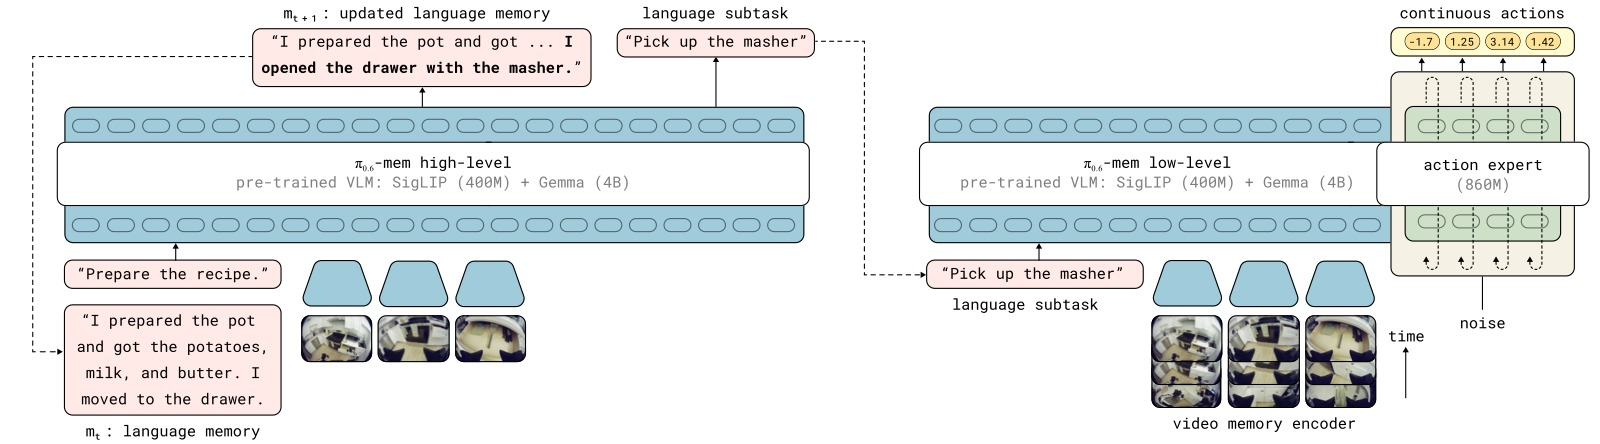
\includegraphics[width=\linewidth]{figures/system_overview.pdf}
    \caption{\small{The \Acronym{} memory system equips VLAs like \pizerosix{} with long-horizon memory via two key components: (1)~a high-level policy is trained to keep track of \textbf{long-horizon} semantic events by updating a \textbf{language memory} $m_t$ (left, \cref{sec:language_memory}), (2)~the low-level policy uses a \textbf{short-horizon} observation-based memory that is efficiently encoded via a \textbf{video encoder} (right, \cref{sec:video_encoder}).}}
    \label{fig:system_overview}
\end{figure*}

\cref{fig:system_overview} shows an overview of our \Acronym{} system.
Our goal is to train a policy $\pi(a_{t:t+H} | o_{t-T:t}, g)$ that predicts a chunk of continuous robot actions $a_{t:t+H}$ conditioned on the task goal $g$ in natural language, as well as a \emph{sequence} of dense observations (e.g. images, proprioceptive state) provided as input.
In comparison, most previous VLAs only condition on a single observation $o_t$, while we want the policy to process many ($T$) observations.

As mentioned above, scaling the number of past observations such that they span multiple minutes, and can thus serve as a form of long-range memory is infeasible.
Therefore, we factorize the problem of action prediction as follows:
\begin{align*}
 	\pi(a_{t:t+H},&\,l_{t+1}, m_{t+1} | o_{t-T:t}, m_t, g) \notag \\
 	\approx~&\pi_\text{LL}(a_{t:t+H} | o_{t-K:t}, l_{t+1}, g) \\
    &\pi_\text{HL}(l_{t+1}, m_{t+1} | o_{t}, m_{t}, g),
\end{align*}
where we separated the probability of actions into a low-level policy $\pi_\text{LL}$ and high-level policy $\pi_\text{HL}$.
The low-level policy models sequences of actions conditioned on the task goal $g$, a shorter sequence of observations ($K \ll T$) and a subtask instruction $l_{t+1}$.
The subtask instruction, in turn, is generated by the high-level policy, which is not only conditioned on the task goal, but also a summarization $m_t$ of previous semantic events in natural language.
We call this summarization the \emph{language memory} in the following.
It allows us to significantly reduce the number $K\ll T$ of dense observations that are input to the model, without sacrificing the ability to capture memory on the order of many minutes.
While previous work has employed a similar split into high- and low-level policies with subtask instructions as the interface, the key novelty here is that $\pi_\text{HL}$ additionally predicts the updated language memory $m_{t+1}$ based on its own previous prediction $m_t$.







\subsection{Language Memory for Long-Term Memory}
\label{sec:language_memory}
The language memory $m_t$ is a summary of previous \emph{semantic} events that happened while the policy is solving a task.
The main idea is to train the high-level policy $\pi_\text{HL}(l_{t+1}, m_{t+1} | o_{t-K:t}, m_{t}, g)$ such that it predicts the relevant summary $m_{t+1}$ from its previous summary $m_t$ and current observations and task.
This way, the model explicitly decides when and how to update its memory representation. For example, for a kitchen cleaning robot that already placed a plate in the cabinet and just finished picking up the next bowl, a memory update may look like the following:

\begin{center}
$m_t$: \small\texttt{I placed a plate in the cabinet and moved to the counter.}

\vspace{5pt}
$\Big\Downarrow$
\vspace{5pt}

$m_{t+1}$: \small\texttt{I placed a plate in the cabinet, moved to the counter, and picked up a bowl.}\hspace{-3pt}
\end{center}

In order to train $\pi_\text{HL}$, we need to obtain appropriate training data, including summarization actions we want the high-level policy to take. For this, we develop a pipeline to generate training data for the transition between $m_t$ and $m_{t+1}$ as follows.
Given a robot episode with subtask language annotations $l_{0:T}$, we pass the subtask instructions together with an indicator whether the subtask execution failed or succeeded to an off-the-shelf pre-trained language model (LLM) and ask it to summarize all information from the previous subtasks that is still relevant for future task execution. We collect the corresponding output and use it to label the sequence for training the high-level policy.

Importantly, we instruct the LLM to \emph{remove} or \emph{compress} information in the language memory whenever appropriate. For example, instead of remembering the precise attributes of all objects that were manipulated (``\texttt{I put a light green bowl, a dark blue bowl and a bright yellow bowl into the top right cabinet}''), it is often sufficient to just remember where the bowls were placed (``\texttt{I placed three bowls in the top right cabinet}''). Compressing the language memory helps keep it succinct (and thus inference fast) and reduces the potential for train-inference distribution shift, since fewer bits of information are carried over between timesteps. We find that current generation LLMs are effective at this task when prompted to keep only the minimal set of relevant information.



\subsection{Video Encoder for Dense Short-Term Visual Memory}
\label{sec:video_encoder}

\begin{figure}
    \centering
    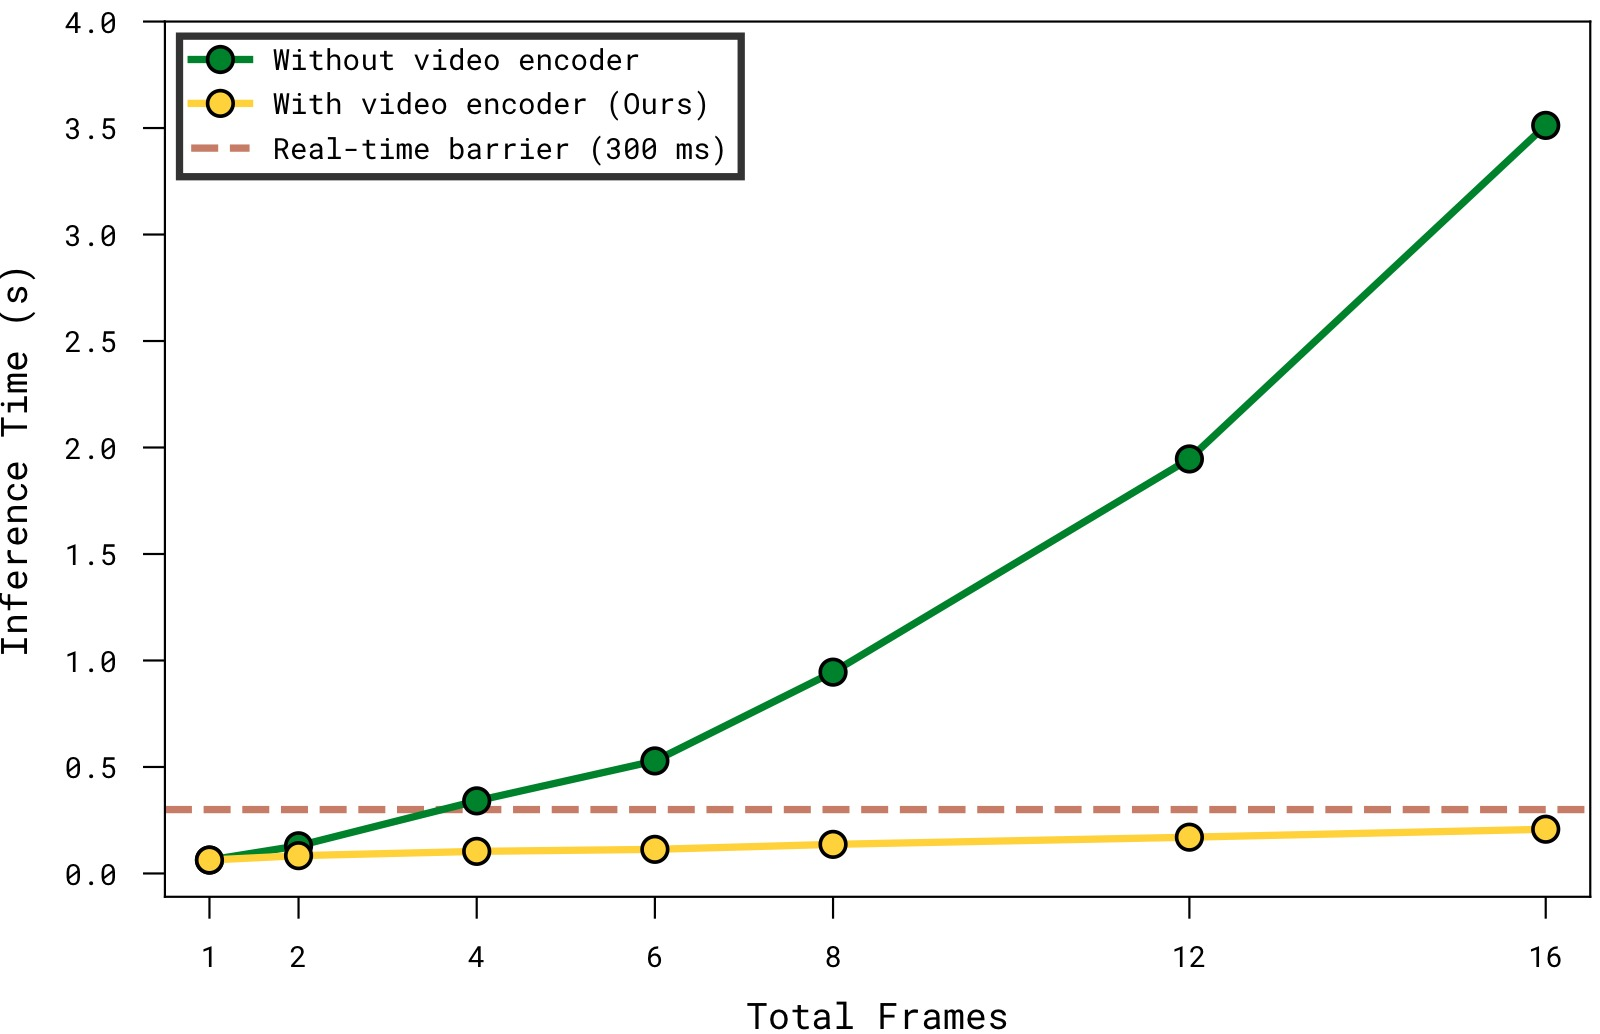
\includegraphics{figures/inference_speed.pdf}
    \caption{\small{Naively passing a sequence of observations into the backbone of a VLA rapidly increases inference latency. Our efficient video encoder architecture allows us to use many observation frames while remaining under critical real-time inference thresholds \cite{black2025real,black2025training}. Timings measured for the \pizerosix{} VLA, with four input camera streams on one NVIDIA H100 GPU.}}
    \label{fig:inference_time}
\end{figure}


The language memory mechanism, as described in the last section, can capture long-term \emph{semantic} concepts.
In order to enable our policies to reason about fine-grained details, dynamics, and resolve self-occlusion, access to a dense sequence of previous observations $o_{t-K:t}$ is required as input to the policy.
In most VLAs, encoding the observations, especially for images, accounts for the largest fraction of compute spent during training and significantly impacts inference speed.
Therefore, as we show in \cref{fig:inference_time}, simply encoding a sequence of observations one-by-one and passing them into the VLA backbone quickly becomes infeasible as the context grows beyond a few timesteps. The VLA will rapidly incur inference latencies beyond what prior work has deemed acceptable to prevent significant degradation in on-robot performance for dexterous manipulation tasks~\citep{black2025real, black2025training}.

\begin{figure}
    \centering
    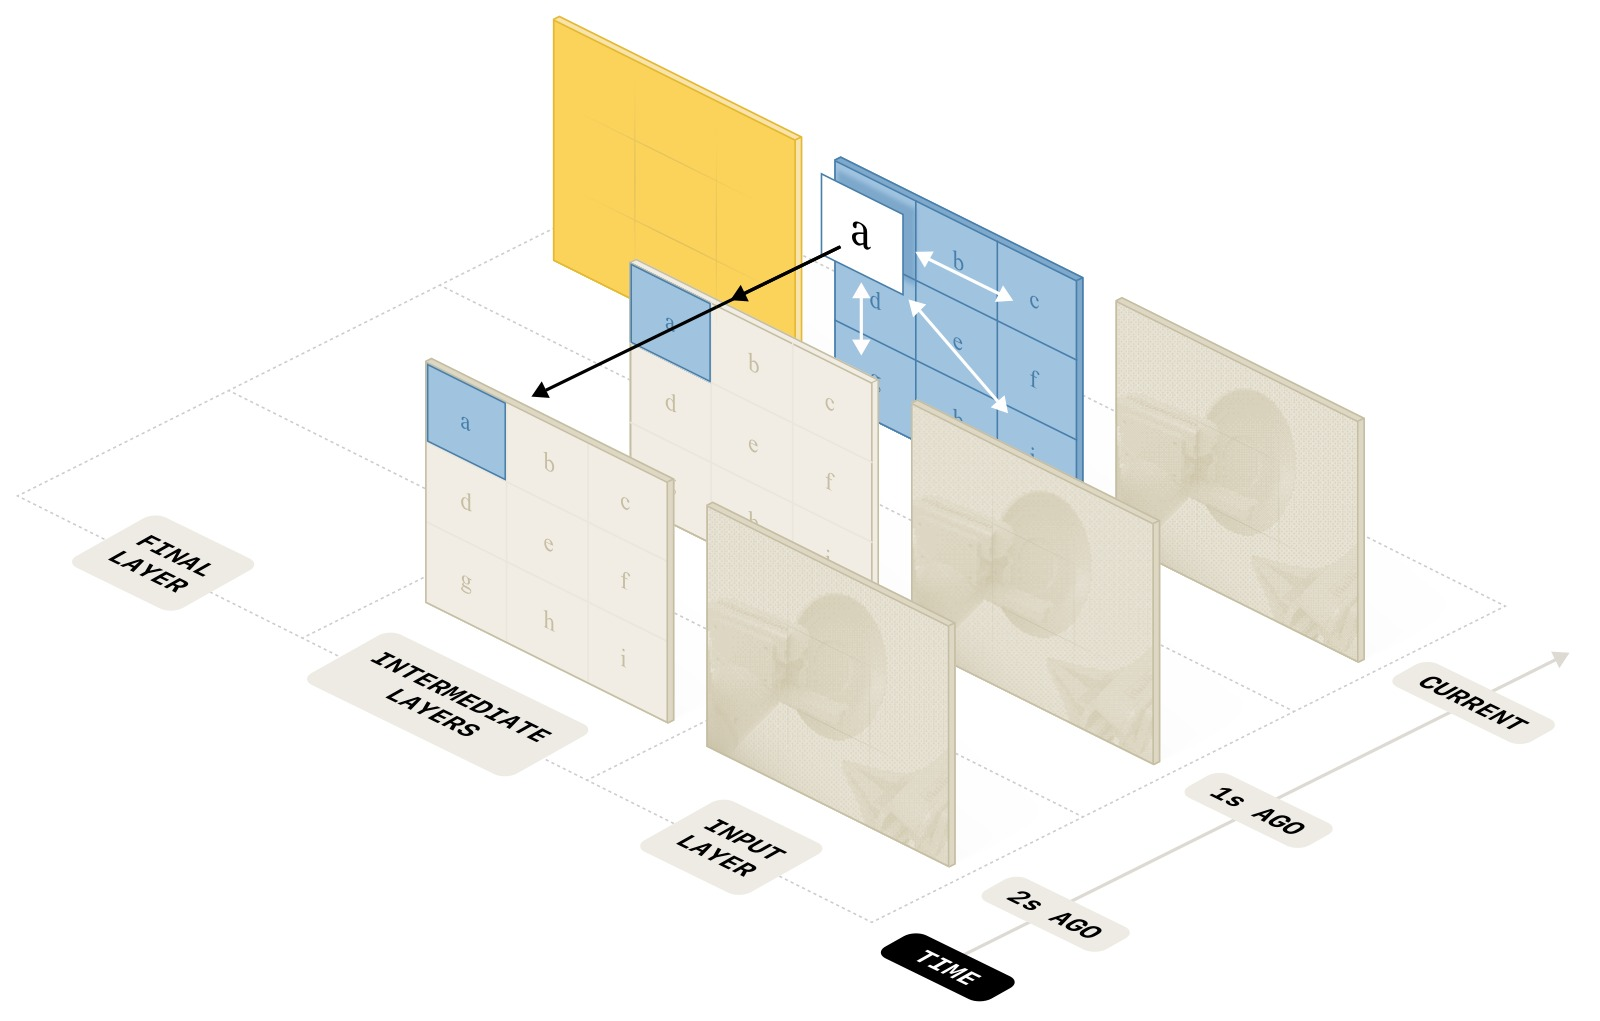
\includegraphics[width=\linewidth]{figures/video_encoderv5.pdf}
    \caption{\small{We propose to use an efficient video encoder architecture for compressing short-horizon, image-based memory. Our architecture expands standard ViTs for encoding video inputs by interleaving layers that apply bidirectional spatial attention \emph{within} each observation (white arrows) with layers that additionally apply causal-temporal attention operations \emph{across} observations (black arrows). We drop observation tokens for past timesteps in upper layers of the ViT to compress the inputs and reduce the number of tokens passed to the VLA backbone.}}
    \label{fig:video_encoder}
\end{figure}


To address this, we propose to use a video encoder that can compress frames in the time dimension before passing the encoding into the VLM backbone.
Our video encoder extends Vision Transformers (ViTs)~\citep{dosovitskiy2020image}, typically used as the vision encoder in most VLAs, to encode video inputs.
Importantly, our encoder leaves the single-image performance of the VLM we start with invariant, and thus can be used to endow any pre-trained VLM with highly effective (yet computationally cheap) visual memory capabilities.


ViTs process images in patches and repeatedly perform bidirectional attention across the patch embeddings (across multiple layers) to derive a final set of output embeddings.
We keep the same general structure and our video encoder first patchifies all images in the input video separately. Inspired by existing work on space-time separable attention for video understanding (see e.g. \citet{bertasius2021space} for an overview) we then modify the attention mechanism every 4-th layer of the ViT to incorporate both spatial (as is standard in ViTs) but also temporal context. To avoid prohibitively expensive joint attention operations over the very large number of total patches in time and space, our architecture factorizes attention into separate \emph{spatial} and \emph{temporal} attention operations.
Every 4-th layer additively adds attention over the time dimension by performing attention over the timesteps' representations for \emph{the same} image patch using a causal attention mask (``temporal'') -- see \cref{fig:video_encoder} for a visual depiction and Appendix \ref{appendix:st_attention} for a mathematical description. 
This reduces the computational complexity of the corresponding attention in each layer from $\mathcal{O}(n^2K^2)$ (for naive attention over both time and space) to $\mathcal{O}(Kn^2 + n K^2)$.
Finally, to reduce the number of patches processed by the subsequent VLA transformer backbone, we only pass the representation computed for the current timestep onwards (dropping representations for all patches from past timesteps).
Thus, our video encoder \emph{matches} the number of tokens typically passed into the VLA backbone in single-timestep VLAs without memory; and we effectively force the video-encoder to incorporate temporal information into the representation produced for the current observation (via the modified attention mechanism).

A key property of our video encoder is that it \emph{does not} introduce new learnable parameters compared to standard, single-image ViTs. Video encoding capabilities are added by modifying the \emph{attention pattern} of the ViT and adding a fixed sinusoidal temporal position encoding. Thus, we can initialize the weights of our video encoder from the pre-trained ViT weights of any standard vision-language-models, just like in no-memory VLAs.
To maximize feature transfer, we ensure that for $K = 1$, i.e., single-image input, our encoder's initialization \emph{exactly} matches that of the VLM, which we achieve with a sinusoidal temporal position embedding that has value $0$ for $t = 0$.

In summary, our video encoder architecture allows us to effectively scale observation-based memory to tens of seconds without incurring prohibitive computational overhead during training or inference (\cref{fig:inference_time}), while at the same time permitting initialization from pre-trained vision-language model weights.









\subsection{Integrating \Acronym{} into the \pizerosix{} VLA}
\label{sec:memory_vla}

For our experimental evaluation, we equip the \pizerosix{} VLA~\cite{intelligence2025pi} with \Acronym{} memory by adapting its architecture to support the video encoder from \cref{sec:video_encoder}.
Like \pizerosix{}, the \pizerosix{} VLA with \Acronym{} is initialized from a pre-trained Gemma3-4B VLM~\citep{kamath2025gemma}.
Following~\citet{driess2025knowledge}, the model is trained with both discrete FAST action token prediction~\citep{pertsch2025fast} and a flow-matching action expert~\citep{blackpi0} with 860M parameters.
Gradients don't flow from the action expert into the VLM backbone~\citep{driess2025knowledge}. The model is trained with an input resolution of 448x448~px per camera stream and up to four camera streams (depending on the robot embodiment).

In addition to past camera frames, the observation memory of the \pizerosix{} model with \Acronym{} memory also contains past proprioceptive states, e.g., joint angles. The \pizerosix{} VLA represents the robot's state in text form. However, in the case of a \emph{sequence} of past states, this would quickly lead to a very large number of state text tokens. 
To prevent this, we instead use a continuous state embedding by projecting each proprioceptive state into the backbone embedding space with a linear projection.
This way, we only produce $K$ proprioceptive state tokens for an observation memory of length $K$.

We pre-train \pizerosix{}-\Acronym{} on a diverse mixture of data that includes teleoperated robot demonstrations, policy rollout data, and human corrections similarly to \citet{intelligence2025pi}, vision-language tasks, and \emph{video}-language tasks, such as video captioning.
During pre-training, we train the model with a sequence of six observations (five past and the current observation), spaced with a stride of one second.
During post-training, we find that we can flexibly expand this horizon and accommodate much longer observation-based memory (up to 18~frames and 54~seconds of observation-based memory in our experiments), similarly to what has been observed in language model and vision-language model training~\citep{chen2023extending}. 
We run all on-robot experiments using either inference-time real-time chunking~(RTC, \citep{black2025real}) or training-time RTC~\citep{black2025training} for asynchronous real-time inference.


























